\documentclass{article}
\usepackage[english]{babel}
\usepackage[utf8]{inputenc}
\usepackage{amsmath}
\usepackage{interval}
%--\usepackage[table]{xcolor}
\usepackage{graphicx}
%--\usepackage{float}
%--\usepackage{longtable}
%--\usepackage{rotating}
%--\usepackage{booktabs}
%--\usepackage{caption}

\usepackage{listings}

\usepackage{hyperref}
\hypersetup{
	colorlinks,
	citecolor=black,
	filecolor=black,
	linkcolor=black,
	urlcolor=black
}

\begin{document}


\begin{titlepage}
      \centering
      \begin{figure}
            \begin{center}
                  
\includegraphics[width=0.6\textwidth]{images/logo_polimi.png}
            \end{center}
      \end{figure}
      \vfill
      {\scshape\LARGE Numerical Analysis for Machine Learning\\Academic Year 2021 - 2022 \par}
      
      
      \vfill
      \newcommand{\HRule}{\rule{\linewidth}{0.3mm}}
      \centering
      \HRule \\[0.4cm]
      \huge  movieRecommendation\\% Title of your document
      \HRule \\
      \vspace{1cm}
      {\Large Sofia \textsc{Martellozzo} \quad Matteo \textsc{Nunziante} \par}
      \vfill
      {\large Professor\par
          Edie \textsc{Miglio}}
\end{titlepage}


\newpage
\renewcommand\contentsname{Contents}
\tableofcontents

\newpage

%------------------------------------------%
\section{Introduction}

With the advent of the internet today, we are witnessing an
enormous information overload. This exponential growth in
data results in difficulty organizing and analyzing this basic
information but opens up new avenues on the paths of
knowledge. The question is no longer to have the information
but to find the relevant information simultaneously; from there,
recommendation systems were born.\\ \\
\textbf{Recommender System} is a system that seeks to predict or filter preferences according to the user’s choices. Recommender systems are utilized in a variety of areas including movies, music, news, books, research articles, search queries, social tags, and products in general. 
Recommender systems produce a list of recommendations in any of the two ways :
\begin{itemize}
      \item \textbf{Collaborative filtering}: Collaborative filtering approaches build a model from the user’s past behavior as well as similar decisions made by other users. This model is then used to predict ratings for items that users may have an interest in.\\
      \begin{figure}[h]
            \begin{center}
                  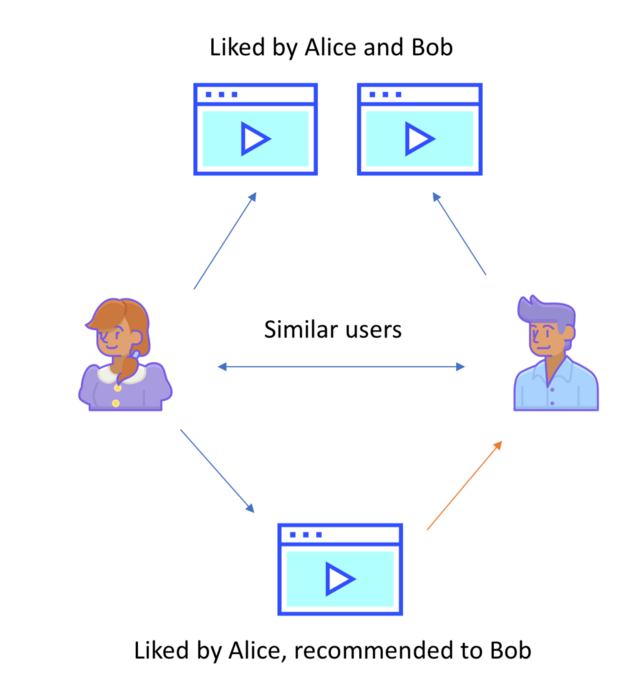
\includegraphics[width=0.5\textwidth]{images/Collaborative filtering.png}
            \end{center}
      \end{figure}\\
      The \underline{advantages} of this approach are:
      \begin{itemize}
            \item Domain knowledge not required: The system does not required a domain knowledge because is based only on item ratings.
            \item Serendipity: The model can help users discover new interests. In isolation, the ML system may not know the user is interested in a given item, but the model might still recommend it because similar users are interested in that item. 
      \end{itemize}
      The \underline{limitations} of this approach are:
      \begin{itemize}
            \item Cold start problem: The prediction of the model for a given (user, item) pair is the dot product of the corresponding embeddings. So, if an item is not seen during training, the system can't create an embedding for it and can't query the model with this item.
            \item Sparsity: The system may find problems on predicting evaluation because of a situation in which the users evaluate a little of the total number of items available in a dataset. This creates a sparse matrix with a high number of missing values.
      \end{itemize}

      \item \textbf{Content-based filtering}: Content-based filtering approaches uses a series of discrete characteristics of an item in order to recommend additional items with similar properties. Content-based filtering methods are totally based on a description of the item and a profile of the user’s preferences. It recommends items based on the user’s past preferences.\\
      \begin{figure}[ht]
            \begin{center}
                  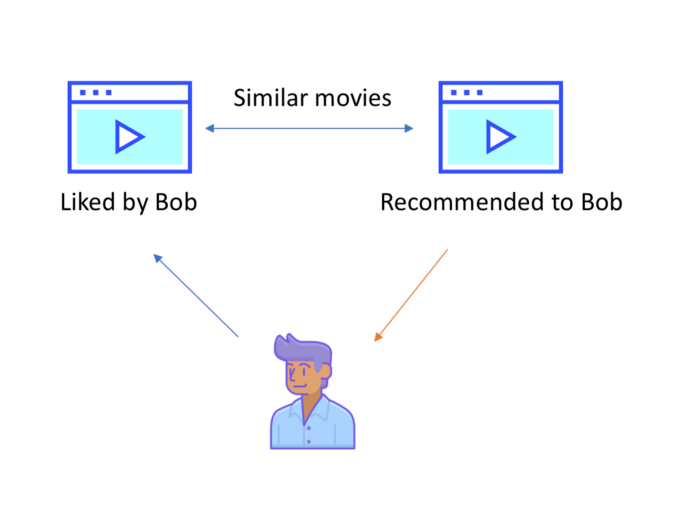
\includegraphics[width=0.5\textwidth]{images/Content-based filtering.png}
            \end{center}
      \end{figure}\\
      The \underline{advantages} of this approach are:
      \begin{itemize}
            \item User autonomy:The model doesn't need any data about other users, since the recommendations are specific to this user. This makes it easier to scale to a large number of users.\\The model can capture the specific interests of a user, and can recommend niche items that very few other users are interested in.
            \item Immediate consideration of a new item: The model does not need the evaluation of all movie by a user, because it can be recommended without being evaluated.
      \end{itemize}
      The \underline{limitations} of this approach are:
      \begin{itemize}
            \item Content too specific: The model can only make recommendations based on existing interests of the user. In other words, the model has limited ability to expand on the users' existing interests.
            \item Big scale information: Since the feature representation of the items are hand-engineered to some extent, this technique requires a lot of domain knowledge. The items must be enouth detailed descripted and a user must evaluate several items before the system can iterpret its preferences.
      \end{itemize}
\end{itemize}
It is also possible to combine these two class of recommendation in order to overcome some limitations they faced. This type of approach is called \textbf{Hybrid Recommendation}.\\
In this project the items that has been avaluated are movies, and their score are the rating that the users gave them, is supposed after they whatched it.

\newpage

%------------------------------------------%
\section{Objectives}

\newpage

%------------------------------------------%
\section{Dataset description}
--Overall description-

\subsection{Movies}
--first dataset--

\subsection{Ratings}
--second dataset--

ADDING: 80\% training and 20\% test

\newpage

%------------------------------------------%
\section{Algorithm description}
--overall description--

\subsection{Binary search}
-- description --
Used to sort the ids of the user and movie for the ratings matrix\\ \\
delate the user that has not whatched any movies\\ \\
built movie-gener matrix M :

\begin{equation}
      M_{i,j} = \left \{
            \begin{aligned}
                  &1 && \text{if movie i is of genre j}\\
                  &0 && \text{otherwise}
            \end{aligned} \right.
\end{equation}

\subsection{Movie-movie similarity}
create a function that calculate the similarity betweeb 2 movies 
use it to create a matrix were movie-movie with the similarity result

Get the two movie from the matrix M like vectors:\\
movie1= $\begin{pmatrix}
      1&0&0&1&0&1
\end{pmatrix}$\\
movie2= $\begin{pmatrix}
      1&1&0&1&0&1
\end{pmatrix}$
\subsubsection{Jaccard similarity coefficient}
It is a statistic index that is used for gauging the similarity and diversity of sample sets, defined by interaction divided by the size of the union of the sample sets:
\begin{equation}
      J(A,B) = \dfrac{|A\cap B|}{|A\cup B|}
\end{equation}
so it is a value between 0 $\leq$ J(A,B) $\leq$ 1
\subsubsection{Cosine similarity}
It gaves a measure of similarity between two non-zero vectors of an inner product space. It calculate the cosine of the angle($\theta$) between them, which is also the same as the inner product of the same vectors normalized to both have lenght 1. \\
\begin{figure}[ht]
      \begin{center}
            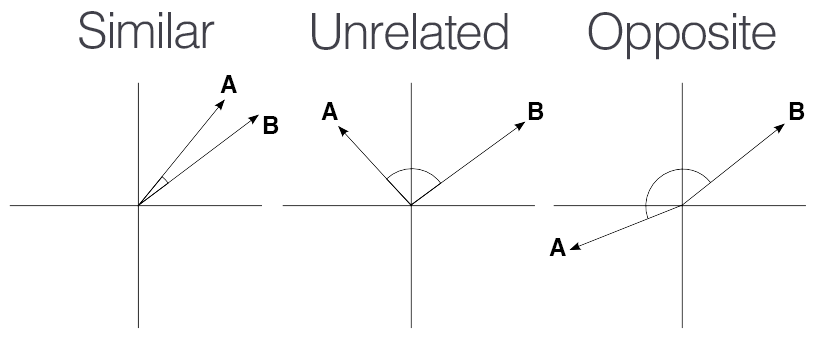
\includegraphics[width=0.7\textwidth]{images/cosine.png}
      \end{center}
\end{figure}\\
Because of that it is bounded in the interval [-1,1] for any angle $\theta$ :
\begin{itemize}
      \item two vectors with the same orientation have a cosine similarity of \textbf{1}
      \item two vectors oriented at right angle relative to each other have a similarity of \textbf{0}
      \item two vectors diametrically opposed have a similarity of \textbf{-1}
\end{itemize}
By using the Euclidean dot product formula:
A $\cdot$ B = $\|A\|$ $\|B\|$ $\cos\theta$ \\
We obtain the cosine similarity formula:\\
\begin{equation}
      S_c(A,B) = \cos\theta = \frac{A \cdot B}{\|A\| \|B\|} = \frac{\sum_{i=1}^n A_i B_i}{\sqrt{\sum_{i=1}^n A_i^2}\sqrt{\sum_{i=1}^n B_i^2}}
\end{equation}\\
where $A_i$ anf $B_i$ are components of vector A and B respectively.


Now create the clusters that contains the similar movies to one and another in it. 

Fill the matrix containing the rating predicting the ones missing:
for each user get all the movies he likes (gave a score $\ge$ 3.5) 
then, from the cluster on which it is contained, get all the movies similar to it and for the ones that haven't been evaluated yet predict the rating of a value equal to the one gave for the original movie.

\subsection{User-user similarity}
Here find the user similar for each other based on the movie both liked, in order to predict a good rating on the film that one user has'nt seen yet but a similar user did.
\subsubsection{SVD}
Perform SVD on the matrix with the origin ratings and the predicred one by content-based filtering approach.\\
In linear algebra, the singular value decomposition (SVD) is a factorization of a real or complex matrix. It generalizes the eigendecomposition of a square normal matrix with an orthonormal eigenbasis to any m × n matrix.
\begin{equation}
      S = U\Sigma V^T
\end{equation}
Specifically, the singular value decomposition of an m $\times$ n complex matrix S is a factorization of the form U$\Sigma V^T$, where \textbf{U} is an m $\times$ m complex unitary matrix, \textbf{$\Sigma$} m $\times$ n rectangular diagonal matrix with non-negative real numbers on the diagonal, and \textbf{V} is an n $\times$ n complex unitary matrix.\\
The diagonal entries $\sigma _{i}$ = $\Sigma _{ii}$ of $\Sigma$ are known as the singular values of S. The number of non-zero singular values is equal to the rank of S. The columns of U and the columns of V are called the left-singular vectors and right-singular vectors of S, respectively.\\
-Filter on the value just lower than the threshold\\
-reconstruct the matrix multiply the tre matrix U a diagonal one with the \\eigenvalues higher than the treshold and V transposed\\


\newpage

%------------------------------------------%
\section{Results}
From the result obtained get an example: from one user, his ratings, the first 10 movie our system would reccommend

\subsection{Error calculation}
From the result obtained compare it with the part of dataser keeped for the testing
\subsubsection{RMSE}
--description--
\subsubsection{rho}
--description--

\subsection{Precision}
--description--
\subsection{Recall}
--description--

\end{document}